\chapter{Resultados \label{chap:Resultados}}
%%%%%%%%%%%%%%%%%%%%%%%%%%%%%%%%%%%%%%%%%%%%%%%%%%%%%%%%%%%%%%%%%%
%%%%%%%%%%%%%%%%%%%%%%%%%%%%%%%%%%%%%%%%%%%%%%%%%%%%%%%%%%%%%%%%%%
\section{Ajuste de espectros}
\noindent Habiendo calculado y aplicado los valores de expectación, $\mu_{g}$ y $\mu_{bkg}$, para corregir la carga sobre los clusters y habiendo introducido el modelo de la colección parcial de carga, que es usado en el ajuste de los espectros, ya se pueden obtener los resultados derivados de las correcciones.

A continuación se presentan los resultados tanto para el pico del flúor como los picos del aluminio. Para ambos casos se muestran los histogramas con sus respectivos ajustes y los resultados para cada uno de los pasos del análisis con el fin de poder comprar los resultados de unos con otros: Primero utilizando el umbral \verb|EPIX = 0.5|, luego aumentando el umbral a \verb|EPIX = 1.5| y sin aplicar las correcciones y, por último, los resultados con el umbral \verb|EPIX = 1.5| aplicando las correcciones.

Para el caso del pico del flúor, se ve en el gráfico de la figura \ref{fig:F_OHDU0_EPIX05} el ajuste del histograma utilizando este modelo para el primer cuadrante del sensor y con \verb|EPIX=0.5|. Se ve como el modelo ajusta muy bien los datos. Además es importante destacar la cantidad de eventos que reconoció el programa fue $677$. 
\begin{figure}[h]
    \centering
        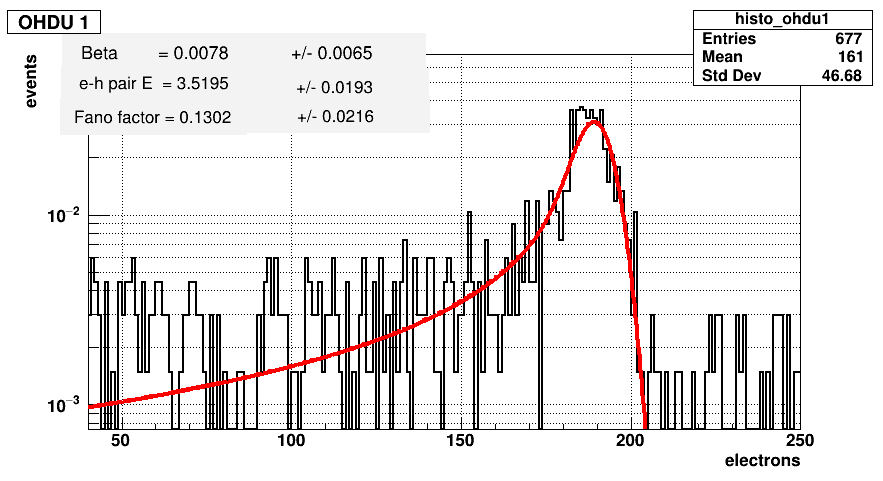
\includegraphics[scale=0.4]{pngs/F_OHDU0_EPIX05.png}
    \caption{\footnotesize{asd.}}
    \label{fig:F_OHDU0_EPIX05}
\end{figure}
De este ajuste se desprenden los valores de los parámetros de interés que son $\beta = 0.0078 \pm 0.0065$, el factor de Fano $F = 0.1302 \pm 0.0216$ y la energía de creación electrón hueco $\eh = 3.5195 \pm 0.0193$.

En el gráfico de la figura \ref{fig:F_OHDU0_EPIX15conCorr} se encuentra el ajuste de los datos para el caso en el que se utilizó el umbral \verb|EPIX=1.5| sin aplicar correcciones. El conteo de eventos en este caso aumentó a $1977$, casi tres veces más que antes.
\begin{figure}[h]
    \centering
        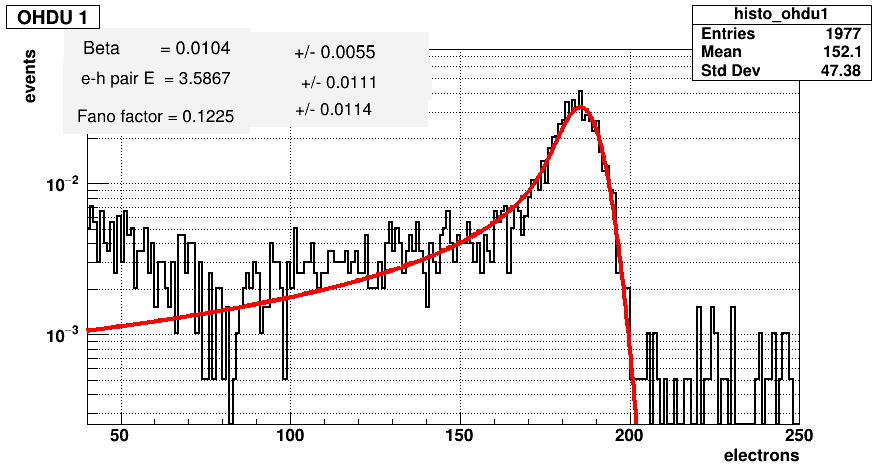
\includegraphics[scale=0.4]{pngs/F_OHDU0_EPIX15_sinCorr.png}
    \caption{\footnotesize{asd.}}
    \label{fig:F_OHDU0_EPIX15sinCorr}
\end{figure}
En este caso aumento se observa un aumento de $\beta$, obteniéndose $\beta = 0.0104 \pm 0.0055$, lo cual también es apreciable en el gráfico porque se observa mayor incidencia de eventos en la cola izquierda del pico. El factor de Fano resultó $F = 0.1225 \pm 0.0114$ y la energía de creación electrón hueco $\eh = 3.5867 \pm 0.0111$. Las incertezas de todos estos parámetros se redujeron sensiblemente respecto al caso anterior con menor estadística.


\begin{figure}[h]
    \centering
        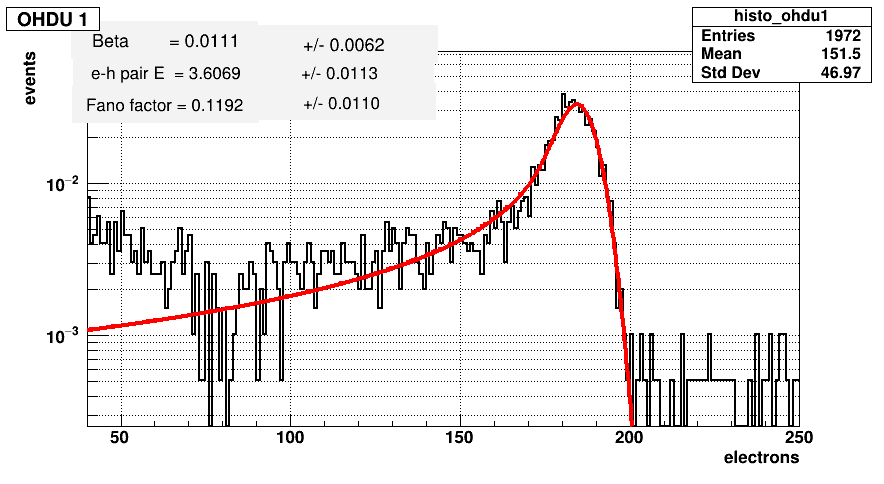
\includegraphics[scale=0.4]{pngs/F_OHDU0_EPIX15_conCorr.png}
    \caption{\footnotesize{asd.}}
    \label{fig:F_OHDU0_EPIX15conCorr}
\end{figure}

En principio se quieren ver los resultados que se obtienen al realizar los ajustes de los picos de los histogramas de carga, para el caso del aluminio, sin aplicar ni el umbral \verb|EPIX = 0.5| ni las correcciones calculadas anteriormente, con el fin de poder comparar resultados. El ajuste puede verse en la figura \ref{fig:Al_OHDU1_EPIX05}, \textit{para el primer cuadrante del sensor}, del cual se obtiene un valor para el factor de Fano de $F = 0.1322 \pm 0.0022$ y la energía de creación electrón hueco $\varepsilon_{\eh} = 3.7141 \pm 0.0019$
\begin{figure}[H]
    \centering
        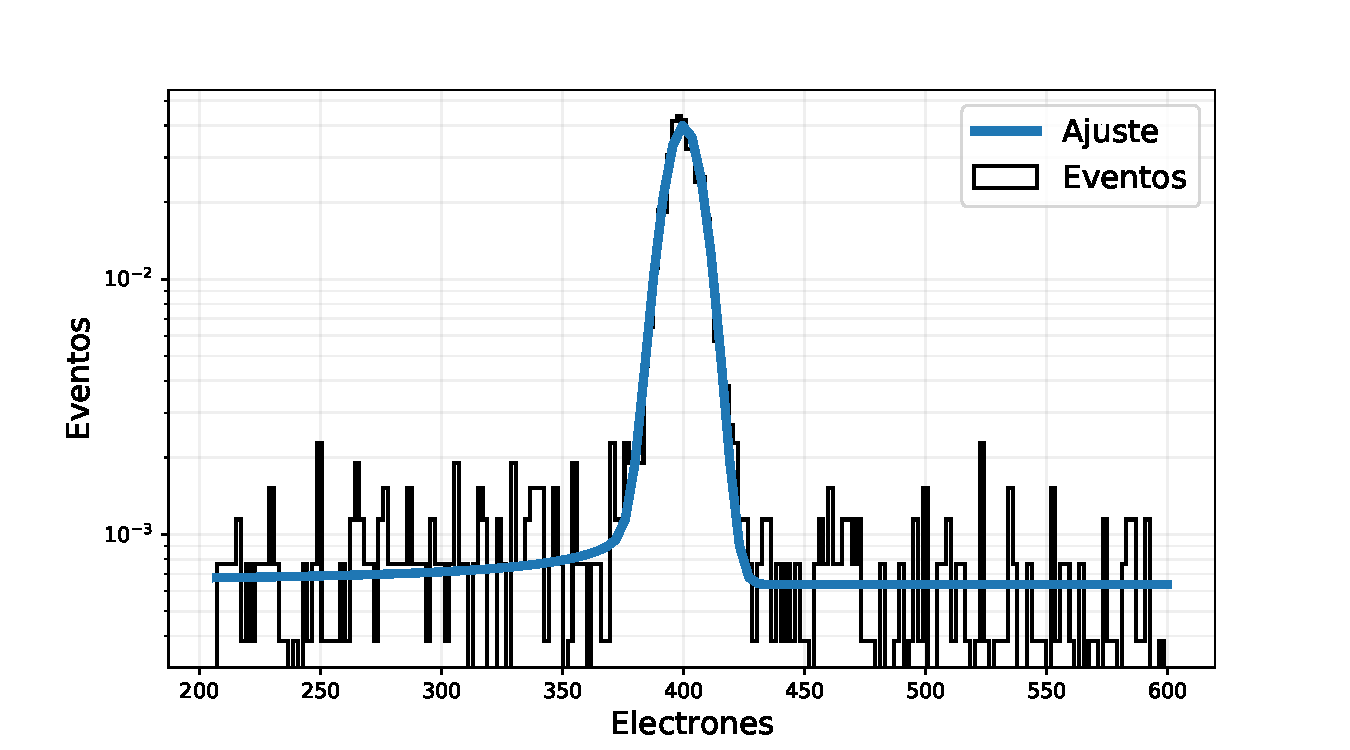
\includegraphics[scale=0.5]{Figs/HistFit_EPIX05_OHDU1_SinCorr.pdf}
    \caption{\footnotesize{asd.}}
    \label{fig:Al_OHDU1_EPIX05}
\end{figure}
Cuando se aplica el umbral con \verb|EPIX|$=1.5$ se eliminan todos los píxeles cuya carga es de un electrón y la estadística del conteo de eventos aumenta, con lo cual se espera una disminución en las incertezas respecto al caso anterior. Se vuelven a generar lo ajustes de los espectros de carga y se desprenden que para factor de Fano se tiene $F = 0.1455 \pm 0.0098$ y para la energía de creación electrón-hueco $\varepsilon_{\eh} = 3.7379 \pm 0.0024$. Lo primero que se observa es que la incerteza del factor de Fano aumenta levemente lo cual es un resultado inesperado. Mismo caso para la energía de creación electrón hueco, donde la incerteza obtenida aumenta sutilmente. Los magnitudes también difieren entre sí más allá de sus errores, un $\sim 10\,\%$ para el factor de Fano y menos del $1\,\%$ para la energía de creación electrón hueco.
\begin{figure}[H]
    \centering
        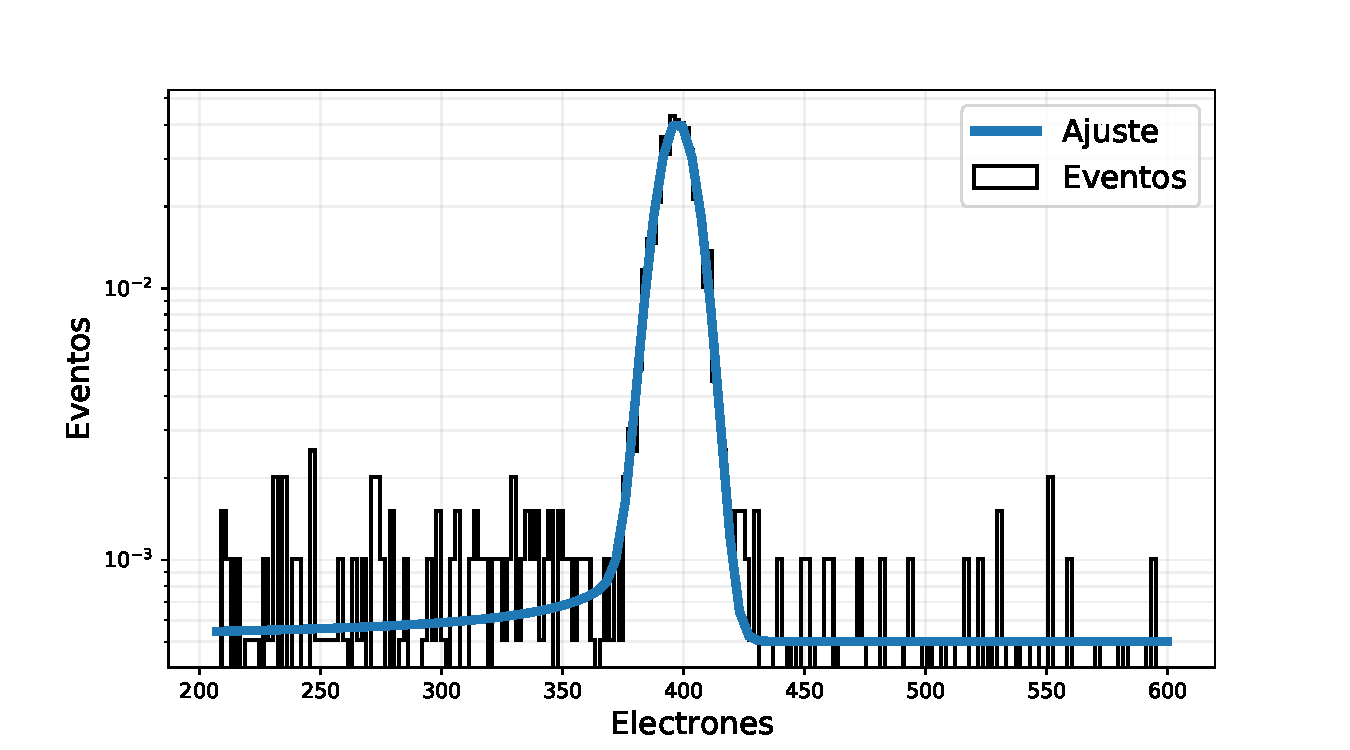
\includegraphics[scale=0.5]{Figs/HistFit_100c_EPIX15_OHDU1_SinCorr.pdf}
    \caption{\footnotesize{asd.}}
    \label{fig:Al_OHDU1_EPIX15_SinCorr}
\end{figure}
Por último, cuando se aplican tanto el umbral como las correcciones en el programa y se generan los ajustes a los histogramas de carga, se esperaría que las incertezas se mantengan y que los valores de las magnitudes varíen levemente. El factor de Fano resultó $F = 0.1450 \pm 0.0037$ y la energía de creación electrón hueco $\varepsilon_{\eh} = 3.7501 \pm 0.0006$. En efecto, se obtienen ligeras variaciones en los valores para el factor de Fano y la energía de creación electrón hueco. En cuanto a las incertezas, estas disminuyen bastante respecto a las anteriormente calculadas y, en particular, la incerteza de la energía de creación electrón hueco es demasiado pequeña.
\begin{figure}[H]
    \centering
        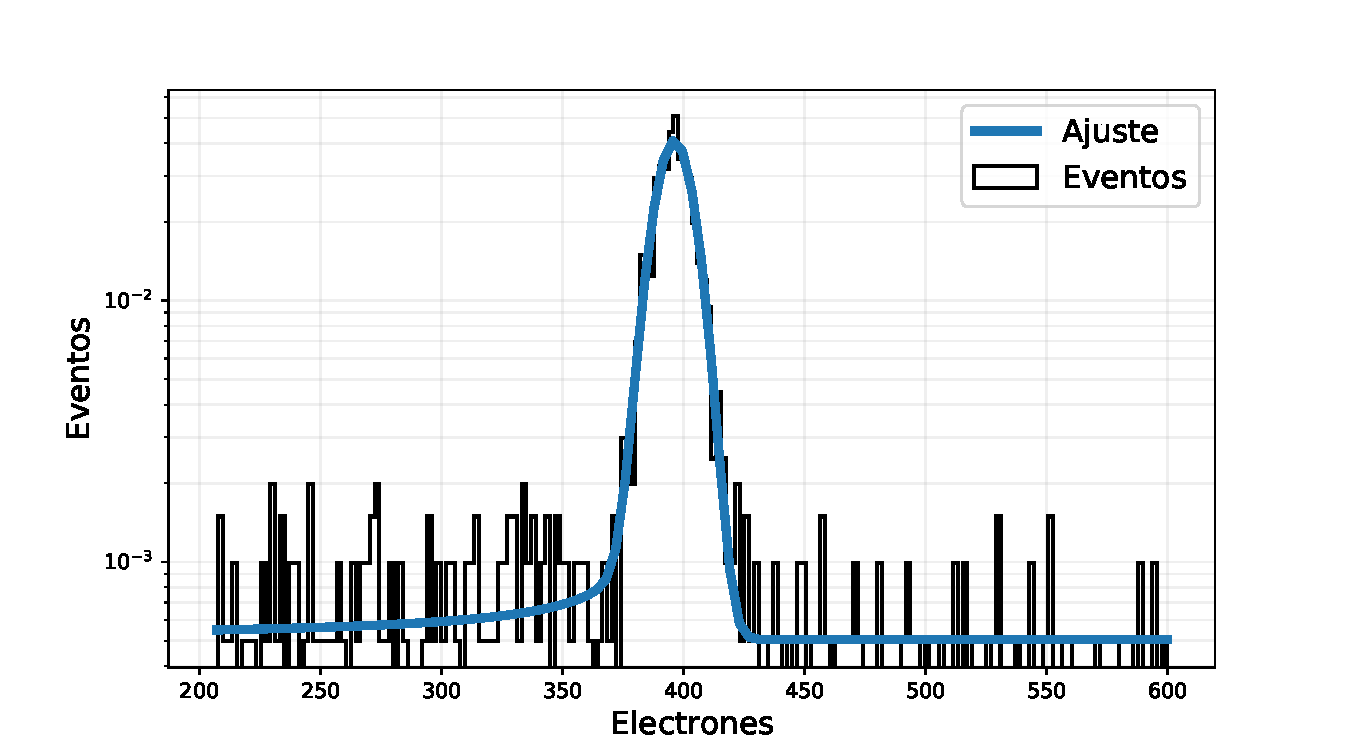
\includegraphics[scale=0.5]{Figs/HistFit_100c_EPIX15_OHDU1_Corr.pdf}
    \caption{\footnotesize{asd.}}
    \label{fig:Al_OHDU1_EPIX15_Corr}
\end{figure}
Los resultados para los demás cuadrantes se muestran en las tablas \ref{tab:FanoEehOHDU1y2} y \ref{tab:FanoEehOHDU3y4}
\begin{table}[H]
\centering
\begin{tabular}{@{}ccccc@{}}
\toprule
                & \multicolumn{2}{c}{OHDU1}                 & \multicolumn{2}{c}{OHDU2}                 \\ \hline\hline
                & $F$                 & $\varepsilon_{\eh}$ & $F$                 & $\varepsilon_{\eh}$ \\
EPIX 0.5 & $0.1322 \pm 0.0022$ & $3.7141 \pm 0.0019$ & $0.1401 \pm 0.0117$ & $3.7149 \pm 0.0037$ \\ \hline
EPIX 1.5 50c & $0.1418 \pm 0.0148$ & $3.7399 \pm 0.0044$ & $0.1339 \pm 0.0186$ & $3.7532 \pm 0.0059$ \\
EPIX 1.5 100c & $0.1455 \pm 0.0098$ & $3.7379 \pm 0.0024$ & $0.1530 \pm 0.0000$ & $3.7386 \pm 0.000$ \\ \hline
EPIX 1.5 50c Corr & $0.1406 \pm 0.0000$ & $3.7490 \pm 0.0000$ & $0.1353 \pm 0.0187$ & $3.7421 \pm 0.0059$ \\
EPIX 1.5 100c Corr & $0.1450 \pm 0.0037$ & $3.7501 \pm 0.0006$ & $0.1513 \pm 0.2640$ & $3.7270 \pm 0.0799$ \\ \bottomrule \hline
\end{tabular}
\caption{tabla}
\label{tab:FanoEehOHDU1y2}
\end{table}
\begin{table}[H]
\centering
\begin{tabular}{@{}ccccc@{}}
\toprule
                & \multicolumn{2}{c}{OHDU3}                 & \multicolumn{2}{c}{OHDU4}                 \\ \hline\hline
                & $F$                 & $\varepsilon_{\eh}$ & $F$                 & $\varepsilon_{\eh}$ \\
EPIX 0.5 & $0.1498 \pm 0.00101$ & $3.7209 \pm 0.0029$ & $0.1812 \pm 0.0166$ & $3.7305 \pm 0.0041$ \\ \hline
EPIX 1.5 50c & $0.1548 \pm 0.0001$ & $3.7449 \pm 0.0000$ & $0.1601 \pm 0.3691$ & $3.7633 \pm 0.1139$ \\
EPIX 1.5 100c & $0.1699 \pm 0.0150$ & $3.7419 \pm 0.0039$ & $0.1931 \pm 0.0208$ & $3.7541 \pm 0.0000$ \\ \hline
EPIX 1.5 50c  Corr& $0.1538 \pm 0.0000$ & $3.7510 \pm 0.0000$ & $0.1487 \pm 0.0000$ & $3.7698 \pm 0.0000$ \\
EPIX 1.5 100c Corr& $0.1701 \pm 0.0141$ & $3.7485 \pm 0.0039$ & $0.1933 \pm 0.0194$ & $3.7634 \pm 0.0047$ \\ \bottomrule \hline
\end{tabular}
\caption{tabla}
\label{tab:FanoEehOHDU3y4}
\end{table}

%%%%%%%%%%%%%%%%%%%%%%%%%%%%%%%%%%%%%%%%%%%%%%%%%%%%%%%%%%%%%%%%%%
%%%%%%%%%%%%%%%%%%%%%%%%%%%%%%%%%%%%%%%%%%%%%%%%%%%%%%%%%%%%%%%%%%
\section{Valores de \texorpdfstring{$\beta$}{beta}}
\noindent Los valores del parámetro $\beta$ junto con su error se determinaron utilizando el método de la máxima verosimilitud como se detalla en la sección \ref{sec:MaximaVerosimilitud}. De realizar este procedimiento se obtuvo el gráfico de la verosimilitud que se ve en la figura \ref{fig:LL_beta} y que se ajustó con una función cuadrática para \textbf{para qué?}. Se puede observar la intersección entre la recta que se encuentra a una distancia $a=1/2$ por debajo del máximo y la curva obtenida del barrido en $\beta$ para la verosimilitud. De estos se obtuvo el intervalo $[0.00396, 0.01144]$ para un $68.3\,\%$ de probabilidad de contener a $beta$, para el \textbf{cual?} cuadrante del sensor y el caso de los rayos $X$ del aluminio.
\begin{figure}[H]
    \centering
        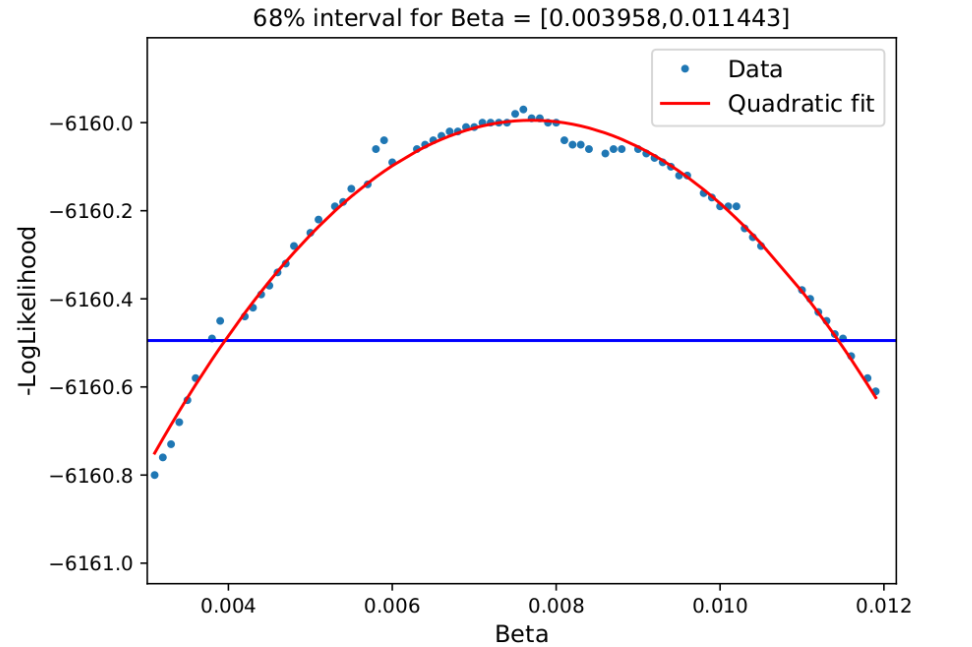
\includegraphics[scale=0.4]{pngs/LL_beta.png}
    \caption{\footnotesize{asd.}}
    \label{fig:LL_beta}
\end{figure}
También se logra observar lo que se esperaba respecto a la intensidad de del parámetro $\beta$: Para los picos de los rayos $X$ del flúor, las colas en los picos de los histogramas son apreciablemente más pronunciadas que para los picos de los rayos $X$ del aluminio. Esto se debe a que $\beta_{F} = 0.008$ mientras que $\beta_{Al} = 0.001$, siendo el efecto de la PCC 8 veces más pronunciado para el caso del flúor.